\documentclass[twoside]{book}

% Packages required by doxygen
\usepackage{fixltx2e}
\usepackage{calc}
\usepackage{doxygen}
\usepackage[export]{adjustbox} % also loads graphicx
\usepackage{graphicx}
\usepackage[utf8]{inputenc}
\usepackage{makeidx}
\usepackage{multicol}
\usepackage{multirow}
\PassOptionsToPackage{warn}{textcomp}
\usepackage{textcomp}
\usepackage[nointegrals]{wasysym}
\usepackage[table]{xcolor}

% Font selection
\usepackage[T1]{fontenc}
\usepackage[scaled=.90]{helvet}
\usepackage{courier}
\usepackage{amssymb}
\usepackage{sectsty}
\renewcommand{\familydefault}{\sfdefault}
\allsectionsfont{%
  \fontseries{bc}\selectfont%
  \color{darkgray}%
}
\renewcommand{\DoxyLabelFont}{%
  \fontseries{bc}\selectfont%
  \color{darkgray}%
}
\newcommand{\+}{\discretionary{\mbox{\scriptsize$\hookleftarrow$}}{}{}}

% Page & text layout
\usepackage{geometry}
\geometry{%
  a4paper,%
  top=2.5cm,%
  bottom=2.5cm,%
  left=2.5cm,%
  right=2.5cm%
}
\tolerance=750
\hfuzz=15pt
\hbadness=750
\setlength{\emergencystretch}{15pt}
\setlength{\parindent}{0cm}
\setlength{\parskip}{3ex plus 2ex minus 2ex}
\makeatletter
\renewcommand{\paragraph}{%
  \@startsection{paragraph}{4}{0ex}{-1.0ex}{1.0ex}{%
    \normalfont\normalsize\bfseries\SS@parafont%
  }%
}
\renewcommand{\subparagraph}{%
  \@startsection{subparagraph}{5}{0ex}{-1.0ex}{1.0ex}{%
    \normalfont\normalsize\bfseries\SS@subparafont%
  }%
}
\makeatother

% Headers & footers
\usepackage{fancyhdr}
\pagestyle{fancyplain}
\fancyhead[LE]{\fancyplain{}{\bfseries\thepage}}
\fancyhead[CE]{\fancyplain{}{}}
\fancyhead[RE]{\fancyplain{}{\bfseries\leftmark}}
\fancyhead[LO]{\fancyplain{}{\bfseries\rightmark}}
\fancyhead[CO]{\fancyplain{}{}}
\fancyhead[RO]{\fancyplain{}{\bfseries\thepage}}
\fancyfoot[LE]{\fancyplain{}{}}
\fancyfoot[CE]{\fancyplain{}{}}
\fancyfoot[RE]{\fancyplain{}{\bfseries\scriptsize Generated by Doxygen }}
\fancyfoot[LO]{\fancyplain{}{\bfseries\scriptsize Generated by Doxygen }}
\fancyfoot[CO]{\fancyplain{}{}}
\fancyfoot[RO]{\fancyplain{}{}}
\renewcommand{\footrulewidth}{0.4pt}
\renewcommand{\chaptermark}[1]{%
  \markboth{#1}{}%
}
\renewcommand{\sectionmark}[1]{%
  \markright{\thesection\ #1}%
}

% Indices & bibliography
\usepackage{natbib}
\usepackage[titles]{tocloft}
\setcounter{tocdepth}{3}
\setcounter{secnumdepth}{5}
\makeindex

% Hyperlinks (required, but should be loaded last)
\usepackage{ifpdf}
\ifpdf
  \usepackage[pdftex,pagebackref=true]{hyperref}
\else
  \usepackage[ps2pdf,pagebackref=true]{hyperref}
\fi
\hypersetup{%
  colorlinks=true,%
  linkcolor=blue,%
  citecolor=blue,%
  unicode%
}

% Custom commands
\newcommand{\clearemptydoublepage}{%
  \newpage{\pagestyle{empty}\cleardoublepage}%
}

\usepackage{caption}
\captionsetup{labelsep=space,justification=centering,font={bf},singlelinecheck=off,skip=4pt,position=top}

%===== C O N T E N T S =====

\begin{document}

% Titlepage & ToC
\hypersetup{pageanchor=false,
             bookmarksnumbered=true,
             pdfencoding=unicode
            }
\pagenumbering{alph}
\begin{titlepage}
\vspace*{7cm}
\begin{center}%
{\Large Arkav\+Quarium }\\
\vspace*{1cm}
{\large Generated by Doxygen 1.8.15}\\
\end{center}
\end{titlepage}
\clearemptydoublepage
\pagenumbering{roman}
\tableofcontents
\clearemptydoublepage
\pagenumbering{arabic}
\hypersetup{pageanchor=true}

%--- Begin generated contents ---
\chapter{Hierarchical Index}
\section{Class Hierarchy}
This inheritance list is sorted roughly, but not completely, alphabetically\+:\begin{DoxyCompactList}
\item \contentsline{section}{Aquarium}{\pageref{class_aquarium}}{}
\item \contentsline{section}{Aquarium\+Object}{\pageref{class_aquarium_object}}{}
\begin{DoxyCompactList}
\item \contentsline{section}{Coin}{\pageref{class_coin}}{}
\item \contentsline{section}{Fish\+Food}{\pageref{class_fish_food}}{}
\item \contentsline{section}{Guppy}{\pageref{class_guppy}}{}
\item \contentsline{section}{Piranha}{\pageref{class_piranha}}{}
\item \contentsline{section}{Snail}{\pageref{class_snail}}{}
\end{DoxyCompactList}
\item \contentsline{section}{Fish}{\pageref{class_fish}}{}
\begin{DoxyCompactList}
\item \contentsline{section}{Guppy}{\pageref{class_guppy}}{}
\item \contentsline{section}{Piranha}{\pageref{class_piranha}}{}
\end{DoxyCompactList}
\item \contentsline{section}{Linked\+List$<$ T $>$}{\pageref{class_linked_list}}{}
\item \contentsline{section}{Linked\+List$<$ Coin $>$}{\pageref{class_linked_list}}{}
\item \contentsline{section}{Linked\+List$<$ Fish\+Food $>$}{\pageref{class_linked_list}}{}
\item \contentsline{section}{Linked\+List$<$ Guppy $>$}{\pageref{class_linked_list}}{}
\item \contentsline{section}{Linked\+List$<$ Piranha $>$}{\pageref{class_linked_list}}{}
\item \contentsline{section}{Node$<$ T $>$}{\pageref{class_node}}{}
\item \contentsline{section}{Node$<$ Coin $>$}{\pageref{class_node}}{}
\item \contentsline{section}{Node$<$ Fish\+Food $>$}{\pageref{class_node}}{}
\item \contentsline{section}{Node$<$ Guppy $>$}{\pageref{class_node}}{}
\item \contentsline{section}{Node$<$ Piranha $>$}{\pageref{class_node}}{}
\end{DoxyCompactList}

\chapter{Class Index}
\section{Class List}
Here are the classes, structs, unions and interfaces with brief descriptions\+:\begin{DoxyCompactList}
\item\contentsline{section}{\mbox{\hyperlink{class_aquarium}{Aquarium}} }{\pageref{class_aquarium}}{}
\item\contentsline{section}{\mbox{\hyperlink{class_aquarium_object}{Aquarium\+Object}} }{\pageref{class_aquarium_object}}{}
\item\contentsline{section}{\mbox{\hyperlink{class_coin}{Coin}} }{\pageref{class_coin}}{}
\item\contentsline{section}{\mbox{\hyperlink{class_fish}{Fish}} }{\pageref{class_fish}}{}
\item\contentsline{section}{\mbox{\hyperlink{class_fish_food}{Fish\+Food}} }{\pageref{class_fish_food}}{}
\item\contentsline{section}{\mbox{\hyperlink{class_guppy}{Guppy}} }{\pageref{class_guppy}}{}
\item\contentsline{section}{\mbox{\hyperlink{class_linked_list}{Linked\+List$<$ T $>$}} }{\pageref{class_linked_list}}{}
\item\contentsline{section}{\mbox{\hyperlink{class_node}{Node$<$ T $>$}} }{\pageref{class_node}}{}
\item\contentsline{section}{\mbox{\hyperlink{class_piranha}{Piranha}} }{\pageref{class_piranha}}{}
\item\contentsline{section}{\mbox{\hyperlink{class_snail}{Snail}} }{\pageref{class_snail}}{}
\end{DoxyCompactList}

\chapter{Class Documentation}
\hypertarget{class_aquarium}{}\section{Aquarium Class Reference}
\label{class_aquarium}\index{Aquarium@{Aquarium}}
\subsection*{Private Attributes}
\begin{DoxyCompactItemize}
\item 
\mbox{\Hypertarget{class_aquarium_a480db476e4c62948bc803371a3a57708}\label{class_aquarium_a480db476e4c62948bc803371a3a57708}} 
int {\bfseries x}
\item 
\mbox{\Hypertarget{class_aquarium_a141ee2e1296df314fefc07407d50d56a}\label{class_aquarium_a141ee2e1296df314fefc07407d50d56a}} 
int {\bfseries y}
\end{DoxyCompactItemize}
\subsection*{Static Private Attributes}
\begin{DoxyCompactItemize}
\item 
\mbox{\Hypertarget{class_aquarium_a9ed1bde466f595a1ed92f5443d0f8efd}\label{class_aquarium_a9ed1bde466f595a1ed92f5443d0f8efd}} 
static const int {\bfseries M\+A\+X\+\_\+X} = 100
\item 
\mbox{\Hypertarget{class_aquarium_a391505700de06b370655b379cc5b0421}\label{class_aquarium_a391505700de06b370655b379cc5b0421}} 
static const int {\bfseries M\+A\+X\+\_\+Y} = 100
\end{DoxyCompactItemize}


The documentation for this class was generated from the following file\+:\begin{DoxyCompactItemize}
\item 
/media/malfianrasyidin/\+A\+L\+F\+I\+A\+N/c++/\+Arkav\+Quarium/src/Arkav\+Quarium.\+hpp\end{DoxyCompactItemize}

\hypertarget{class_aquarium_object}{}\section{Aquarium\+Object Class Reference}
\label{class_aquarium_object}\index{Aquarium\+Object@{Aquarium\+Object}}


Inheritance diagram for Aquarium\+Object\+:\nopagebreak
\begin{figure}[H]
\begin{center}
\leavevmode
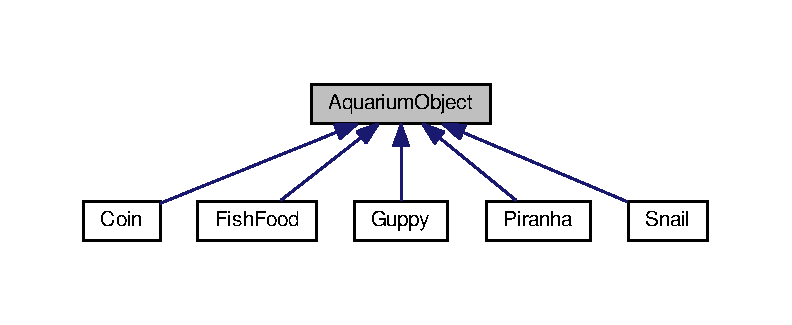
\includegraphics[width=350pt]{class_aquarium_object__inherit__graph}
\end{center}
\end{figure}
\subsection*{Public Member Functions}
\begin{DoxyCompactItemize}
\item 
\mbox{\Hypertarget{class_aquarium_object_a42c4de640f89ac8aebc26b7618578575}\label{class_aquarium_object_a42c4de640f89ac8aebc26b7618578575}} 
virtual void {\bfseries move} ()=0
\item 
\mbox{\Hypertarget{class_aquarium_object_a1dd18ba4c21c8fb1c0796791f527a257}\label{class_aquarium_object_a1dd18ba4c21c8fb1c0796791f527a257}} 
int {\bfseries getX} () const
\item 
\mbox{\Hypertarget{class_aquarium_object_a53eadc1189fa466e61b5f6b2b597de4b}\label{class_aquarium_object_a53eadc1189fa466e61b5f6b2b597de4b}} 
int {\bfseries getY} () const
\item 
\mbox{\Hypertarget{class_aquarium_object_a650f8f46f51ca64889fd3e1455f9696c}\label{class_aquarium_object_a650f8f46f51ca64889fd3e1455f9696c}} 
void {\bfseries setX} (int)
\item 
\mbox{\Hypertarget{class_aquarium_object_aa2ee76b48d56edf3b4cc5bcd199f8efe}\label{class_aquarium_object_aa2ee76b48d56edf3b4cc5bcd199f8efe}} 
void {\bfseries setY} (int)
\end{DoxyCompactItemize}
\subsection*{Private Attributes}
\begin{DoxyCompactItemize}
\item 
\mbox{\Hypertarget{class_aquarium_object_a972920a5b11f5ce825983fde33c1af53}\label{class_aquarium_object_a972920a5b11f5ce825983fde33c1af53}} 
int {\bfseries x}
\item 
\mbox{\Hypertarget{class_aquarium_object_a823e2b6e65e5dc1d650af83097eac427}\label{class_aquarium_object_a823e2b6e65e5dc1d650af83097eac427}} 
int {\bfseries y}
\end{DoxyCompactItemize}


The documentation for this class was generated from the following file\+:\begin{DoxyCompactItemize}
\item 
/media/malfianrasyidin/\+A\+L\+F\+I\+A\+N/c++/\+Arkav\+Quarium/src/Arkav\+Quarium.\+hpp\end{DoxyCompactItemize}

\hypertarget{class_coin}{}\section{Coin Class Reference}
\label{class_coin}\index{Coin@{Coin}}


Inheritance diagram for Coin\+:\nopagebreak
\begin{figure}[H]
\begin{center}
\leavevmode
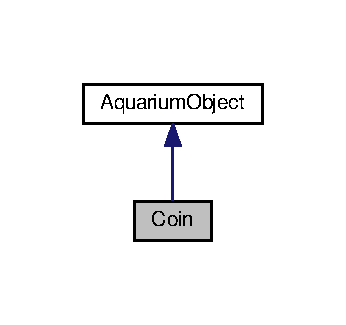
\includegraphics[width=166pt]{class_coin__inherit__graph}
\end{center}
\end{figure}


Collaboration diagram for Coin\+:\nopagebreak
\begin{figure}[H]
\begin{center}
\leavevmode
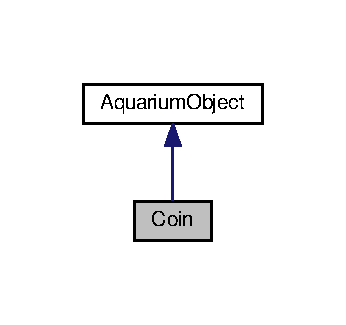
\includegraphics[width=166pt]{class_coin__coll__graph}
\end{center}
\end{figure}
\subsection*{Public Member Functions}
\begin{DoxyCompactItemize}
\item 
\mbox{\Hypertarget{class_coin_ab62bca5834489b9b483deaa3ca3470e9}\label{class_coin_ab62bca5834489b9b483deaa3ca3470e9}} 
void {\bfseries move} ()
\end{DoxyCompactItemize}
\subsection*{Private Attributes}
\begin{DoxyCompactItemize}
\item 
\mbox{\Hypertarget{class_coin_a3273e38e55be31a1c123fc0a46820467}\label{class_coin_a3273e38e55be31a1c123fc0a46820467}} 
int {\bfseries value}
\end{DoxyCompactItemize}


The documentation for this class was generated from the following file\+:\begin{DoxyCompactItemize}
\item 
/media/malfianrasyidin/\+A\+L\+F\+I\+A\+N/c++/\+Arkav\+Quarium/src/Arkav\+Quarium.\+hpp\end{DoxyCompactItemize}

\hypertarget{class_fish}{}\section{Fish Class Reference}
\label{class_fish}\index{Fish@{Fish}}


{\ttfamily \#include $<$Fish.\+hpp$>$}



Inheritance diagram for Fish\+:
\nopagebreak
\begin{figure}[H]
\begin{center}
\leavevmode
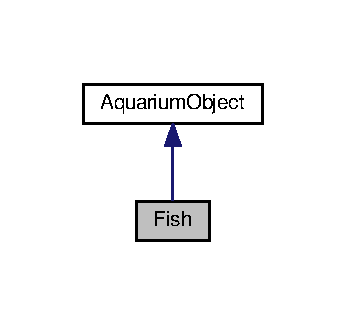
\includegraphics[width=194pt]{class_fish__inherit__graph}
\end{center}
\end{figure}
\subsection*{Public Member Functions}
\begin{DoxyCompactItemize}
\item 
virtual void \mbox{\hyperlink{class_fish_af209980bd39b8de9b4bb38b7ad4edd04}{eat}} ()=0
\item 
\mbox{\Hypertarget{class_fish_a899c7712639756297b9205e8bbcc2cf6}\label{class_fish_a899c7712639756297b9205e8bbcc2cf6}} 
virtual void {\bfseries drop\+Coin} ()=0
\end{DoxyCompactItemize}


\subsection{Detailed Description}
Definisi Kelas Abstrak \mbox{\hyperlink{class_fish}{Fish}} Fungsi\+: Kelas abstrak ini digunakan oleh kelas turunannya yaitu \mbox{\hyperlink{class_guppy}{Guppy}} dan \mbox{\hyperlink{class_piranha}{Piranha}} 

\subsection{Member Function Documentation}
\mbox{\Hypertarget{class_fish_af209980bd39b8de9b4bb38b7ad4edd04}\label{class_fish_af209980bd39b8de9b4bb38b7ad4edd04}} 
\index{Fish@{Fish}!eat@{eat}}
\index{eat@{eat}!Fish@{Fish}}
\subsubsection{\texorpdfstring{eat()}{eat()}}
{\footnotesize\ttfamily virtual void Fish\+::eat (\begin{DoxyParamCaption}{ }\end{DoxyParamCaption})\hspace{0.3cm}{\ttfamily [pure virtual]}}

\mbox{\hyperlink{class_fish_af209980bd39b8de9b4bb38b7ad4edd04}{eat()}} dan drop\+Coin() akan diimplementasikan di kelas anak 

Implemented in \mbox{\hyperlink{class_guppy_afe934262a0988e4ad041f4ed3a1a7e02}{Guppy}}, and \mbox{\hyperlink{class_piranha_ac48c0256edd56c427b3d82f6e0d4df82}{Piranha}}.



The documentation for this class was generated from the following file\+:\begin{DoxyCompactItemize}
\item 
/media/malfianrasyidin/\+A\+L\+F\+I\+A\+N/c++/\+Arkav\+Quarium/src/Fish.\+hpp\end{DoxyCompactItemize}

\hypertarget{class_fish_food}{}\section{Fish\+Food Class Reference}
\label{class_fish_food}\index{Fish\+Food@{Fish\+Food}}


Inheritance diagram for Fish\+Food\+:\nopagebreak
\begin{figure}[H]
\begin{center}
\leavevmode
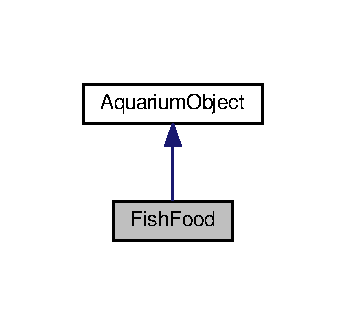
\includegraphics[width=166pt]{class_fish_food__inherit__graph}
\end{center}
\end{figure}


Collaboration diagram for Fish\+Food\+:\nopagebreak
\begin{figure}[H]
\begin{center}
\leavevmode
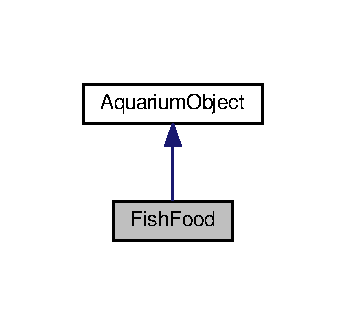
\includegraphics[width=166pt]{class_fish_food__coll__graph}
\end{center}
\end{figure}
\subsection*{Public Member Functions}
\begin{DoxyCompactItemize}
\item 
\mbox{\Hypertarget{class_fish_food_a411070d0e4f5c964ff34ca17fca0ec05}\label{class_fish_food_a411070d0e4f5c964ff34ca17fca0ec05}} 
void {\bfseries move} ()
\end{DoxyCompactItemize}


The documentation for this class was generated from the following file\+:\begin{DoxyCompactItemize}
\item 
/media/malfianrasyidin/\+A\+L\+F\+I\+A\+N/c++/\+Arkav\+Quarium/src/Arkav\+Quarium.\+hpp\end{DoxyCompactItemize}

\hypertarget{class_guppy}{}\section{Guppy Class Reference}
\label{class_guppy}\index{Guppy@{Guppy}}


Inheritance diagram for Guppy\+:
\nopagebreak
\begin{figure}[H]
\begin{center}
\leavevmode
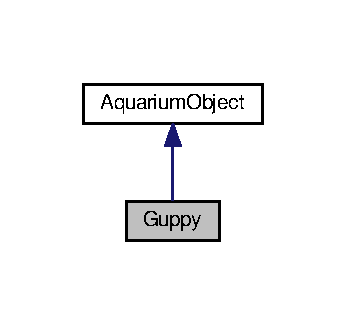
\includegraphics[width=220pt]{class_guppy__inherit__graph}
\end{center}
\end{figure}


Collaboration diagram for Guppy\+:
\nopagebreak
\begin{figure}[H]
\begin{center}
\leavevmode
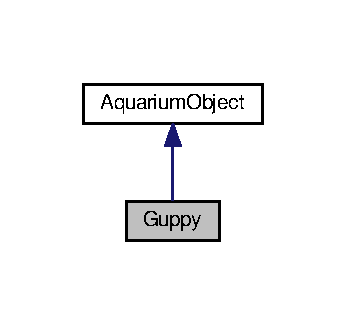
\includegraphics[width=220pt]{class_guppy__coll__graph}
\end{center}
\end{figure}
\subsection*{Public Member Functions}
\begin{DoxyCompactItemize}
\item 
\mbox{\Hypertarget{class_guppy_ae6002948d74b3741bed34a7311be4377}\label{class_guppy_ae6002948d74b3741bed34a7311be4377}} 
void {\bfseries move} ()
\item 
\mbox{\Hypertarget{class_guppy_afe934262a0988e4ad041f4ed3a1a7e02}\label{class_guppy_afe934262a0988e4ad041f4ed3a1a7e02}} 
void {\bfseries eat} ()
\end{DoxyCompactItemize}


The documentation for this class was generated from the following file\+:\begin{DoxyCompactItemize}
\item 
/media/malfianrasyidin/\+A\+L\+F\+I\+A\+N/c++/\+Arkav\+Quarium/src/Guppy.\+hpp\end{DoxyCompactItemize}

\hypertarget{class_linked_list}{}\section{Linked\+List$<$ T $>$ Class Template Reference}
\label{class_linked_list}\index{Linked\+List$<$ T $>$@{Linked\+List$<$ T $>$}}
\subsection*{Public Member Functions}
\begin{DoxyCompactItemize}
\item 
\mbox{\Hypertarget{class_linked_list_a8ef3a028835471b2974552005e621323}\label{class_linked_list_a8ef3a028835471b2974552005e621323}} 
int {\bfseries find} (const \mbox{\hyperlink{class_node}{Node}}$<$ T $>$ \&)
\item 
\mbox{\Hypertarget{class_linked_list_a7ecbb28e82117a680839ed0dc28ebdce}\label{class_linked_list_a7ecbb28e82117a680839ed0dc28ebdce}} 
bool {\bfseries is\+Empty} ()
\item 
\mbox{\Hypertarget{class_linked_list_af2625170c2f18346900058daab78caf0}\label{class_linked_list_af2625170c2f18346900058daab78caf0}} 
void {\bfseries add} (const \mbox{\hyperlink{class_node}{Node}}$<$ T $>$ \&)
\item 
\mbox{\Hypertarget{class_linked_list_aa2d9c914f6b451adbf7f56f4c9c86a6a}\label{class_linked_list_aa2d9c914f6b451adbf7f56f4c9c86a6a}} 
void {\bfseries remove} (const \mbox{\hyperlink{class_node}{Node}}$<$ T $>$ \&)
\item 
\mbox{\Hypertarget{class_linked_list_af640cd5af2af1e91fae857155fd76230}\label{class_linked_list_af640cd5af2af1e91fae857155fd76230}} 
\mbox{\hyperlink{class_node}{Node}} {\bfseries get} (int)
\end{DoxyCompactItemize}


The documentation for this class was generated from the following file\+:\begin{DoxyCompactItemize}
\item 
/media/malfianrasyidin/\+A\+L\+F\+I\+A\+N/c++/\+Arkav\+Quarium/src/Linked\+List.\+hpp\end{DoxyCompactItemize}

\hypertarget{class_node}{}\section{Node$<$ T $>$ Class Template Reference}
\label{class_node}\index{Node$<$ T $>$@{Node$<$ T $>$}}
\subsection*{Public Member Functions}
\begin{DoxyCompactItemize}
\item 
\mbox{\Hypertarget{class_node_a773c2262bb5c0bcea27f3247bbc29fb7}\label{class_node_a773c2262bb5c0bcea27f3247bbc29fb7}} 
T {\bfseries get} ()
\item 
\mbox{\Hypertarget{class_node_a73471424bb2d3e7f7790b812a21588e3}\label{class_node_a73471424bb2d3e7f7790b812a21588e3}} 
void {\bfseries set} (const T \&)
\end{DoxyCompactItemize}


The documentation for this class was generated from the following file\+:\begin{DoxyCompactItemize}
\item 
/media/malfianrasyidin/\+A\+L\+F\+I\+A\+N/c++/\+Arkav\+Quarium/src/Node.\+hpp\end{DoxyCompactItemize}

\hypertarget{class_piranha}{}\section{Piranha Class Reference}
\label{class_piranha}\index{Piranha@{Piranha}}


Inheritance diagram for Piranha\+:
\nopagebreak
\begin{figure}[H]
\begin{center}
\leavevmode
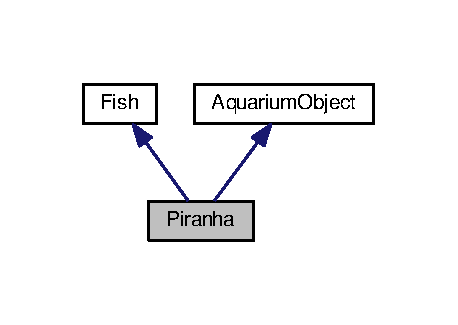
\includegraphics[width=220pt]{class_piranha__inherit__graph}
\end{center}
\end{figure}


Collaboration diagram for Piranha\+:
\nopagebreak
\begin{figure}[H]
\begin{center}
\leavevmode
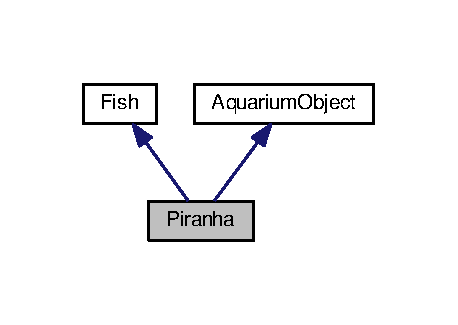
\includegraphics[width=220pt]{class_piranha__coll__graph}
\end{center}
\end{figure}
\subsection*{Public Member Functions}
\begin{DoxyCompactItemize}
\item 
\mbox{\Hypertarget{class_piranha_a6b86e73b3e5a57ee0fdb768c24ab9b67}\label{class_piranha_a6b86e73b3e5a57ee0fdb768c24ab9b67}} 
void {\bfseries move} ()
\item 
\mbox{\Hypertarget{class_piranha_ac48c0256edd56c427b3d82f6e0d4df82}\label{class_piranha_ac48c0256edd56c427b3d82f6e0d4df82}} 
void {\bfseries eat} ()
\end{DoxyCompactItemize}


The documentation for this class was generated from the following file\+:\begin{DoxyCompactItemize}
\item 
/media/malfianrasyidin/\+A\+L\+F\+I\+A\+N/c++/\+Arkav\+Quarium/src/Piranha.\+hpp\end{DoxyCompactItemize}

\hypertarget{class_snail}{}\section{Snail Class Reference}
\label{class_snail}\index{Snail@{Snail}}


Inheritance diagram for Snail\+:\nopagebreak
\begin{figure}[H]
\begin{center}
\leavevmode
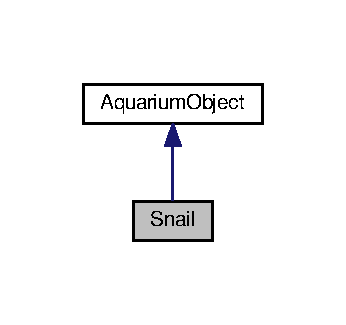
\includegraphics[width=166pt]{class_snail__inherit__graph}
\end{center}
\end{figure}


Collaboration diagram for Snail\+:\nopagebreak
\begin{figure}[H]
\begin{center}
\leavevmode
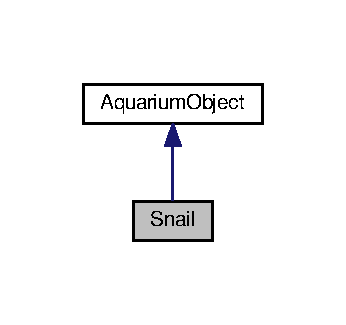
\includegraphics[width=166pt]{class_snail__coll__graph}
\end{center}
\end{figure}
\subsection*{Public Member Functions}
\begin{DoxyCompactItemize}
\item 
\mbox{\Hypertarget{class_snail_af5892ec122d9199480c813b74488256b}\label{class_snail_af5892ec122d9199480c813b74488256b}} 
void {\bfseries move} ()
\item 
\mbox{\Hypertarget{class_snail_a877af082a9bc134a2cd2b4e97c94063d}\label{class_snail_a877af082a9bc134a2cd2b4e97c94063d}} 
void {\bfseries grab\+Coin} ()
\end{DoxyCompactItemize}


The documentation for this class was generated from the following file\+:\begin{DoxyCompactItemize}
\item 
/media/malfianrasyidin/\+A\+L\+F\+I\+A\+N/c++/\+Arkav\+Quarium/src/Snail.\+hpp\end{DoxyCompactItemize}

%--- End generated contents ---

% Index
\backmatter
\newpage
\phantomsection
\clearemptydoublepage
\addcontentsline{toc}{chapter}{Index}
\printindex

\end{document}
